% 1-R² convergence in grid size G — posterior method v3, gamma=0.5, tau=2
\documentclass[border=2mm]{standalone}
\usepackage{pgfplots}
\pgfplotsset{compat=1.18}
\definecolor{red}{rgb}{0.7, 0.11, 0.11}
\definecolor{blue}{rgb}{0.0, 0.20, 0.42}
\definecolor{green}{rgb}{0.11, 0.35, 0.02}
\begin{document}
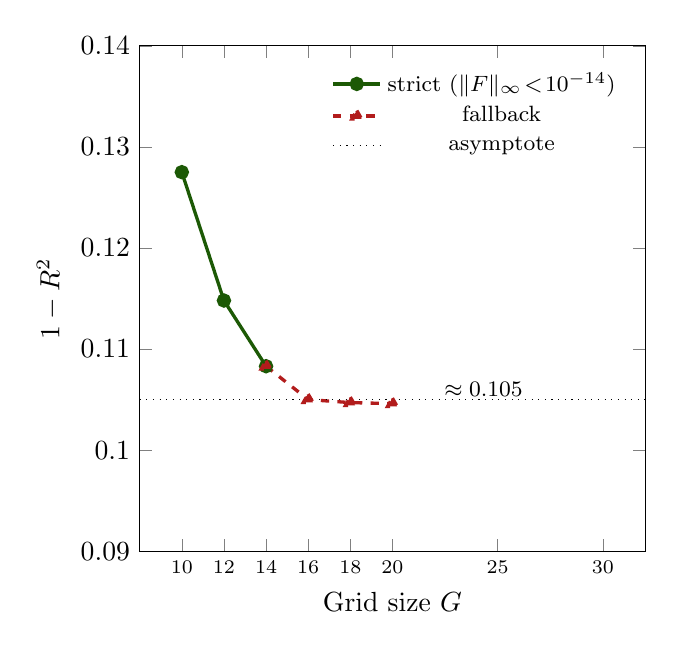
\begin{tikzpicture}
\begin{axis}[
  legend style={draw=none,legend pos=north east,font=\footnotesize},
  ticklabel style={/pgf/number format/fixed,/pgf/number format/precision=5},
  scaled ticks=false,
  ymin=0.09, ymax=0.14, ylabel={$1-R^2$},
  xmin=8, xmax=32,
  xlabel={Grid size $G$},
  xtick={10,12,14,16,18,20,25,30},
  xticklabel style={font=\scriptsize},
  width=8cm, height=8cm,
  title={}]

% Strict convergence (max<=1e-14)
\addplot[very thick,color=green,mark=*,mark size=2pt]
  coordinates {(10,0.1275)(12,0.1148)(14,0.1083)};

% Fallback (converged in value but not in max residual)
\addplot[very thick,color=red,dashed,mark=triangle*,mark size=2pt]
  coordinates {(14,0.1083)(16,0.1050)(18,0.1047)(20,0.1046)};

% Asymptotic level
\addplot[thin,color=black,dotted]
  coordinates {(8,0.105)(32,0.105)};

\node[anchor=west,font=\footnotesize] at (axis cs:22,0.106) {$\approx 0.105$};

\legend{strict ($\|F\|_\infty\!<\!10^{-14}$), fallback, asymptote}

\end{axis}
\end{tikzpicture}
\end{document}
